\chapter{Literature Review}
\label{cha:LitReview}

\section{Why Map the Internet?}
\label{sec:LitReviewWhyMap}

The main aim of this project is to embed a representation of the internet into hyperbolic space and produce a visualisation of this embedding. In order to fully understand why this is useful, we must ask the question: Why do we need a map of the internet? 

Understanding the physical structure of the internet is something that network engineers have to deal with every day, however it can often be difficult to pinpoint problems in networks. For example, in standard Ethernet networks, the presence of a loop can often create a broadcast storm which can render entire parts of a network unusable due to packet flooding. If an accurate map of the network is known in advance then it is possible for an engineer to locate the fault more quickly as they can compare this map to the current state of the network and check to see if any new connections have been added which may be causing the loop. 

While maps may assist engineers on small scale problems they can also assist in diagnosing problems which affect the internet on a more global scale. For example, despite the extreme interconnectedness of the internet it is still possible for a specific node or link to become congested. Congestion of a node or link can cause severe packet loss making data transmission unreliable across the affected area. Having an accurate map of the internet would allow for quick diagnosis of the fault, as well as pinpointing the cause. Though it may have been possible without a map to easily find the affected nodes or links it would be far more difficult to find the cause of the issue. With a map, it is possible to identify features such as a large number of new nodes which may have caused increased data transmission across the affected area. Additionally, a map of the internet with a geographical element may assist in locating pairs of nodes which could receive additional links or additional bandwidth on existing links.

\section{The World Wide Web}

\label{sec:LitReviewWWW}
Munzner et al undertook previous work which consisted of visualising the structure of the World Wide Web (WWW) in hyperbolic space \cite{munzner_visualizing_1995}. Though this may seem similar to the aim of this project there are key differences between the internet and the WWW which distinguish this project. In order to appreciate these differences it is necessary to understand what the WWW is. 

While the internet is a physical concept, the WWW is not. The WWW represents the data that users of the internet can view, specifically it contains text data formatted using the Hypertext Mark-up Language (HTML) standard which allows users to view as well as navigate this data. This is done using a type of application known as a \textit{web browser}. Web browsers allow users to navigate to web addresses (\textit{www.google.co.uk} for example) and view information stored at these addresses. The user views web pages which can also contain links to other web pages, users can follow these links in their browser to visit these other pages. 

If we imagine each web page as a node in a graph and the links between pages as edges then it possible to construct a graph which represents the WWW or a subset thereof. Recall, however that the internet is, at a basic level, a graph too. While these two graphs have similarities they are fundamentally different. While the graph that represents the internet contains at most a single node per physical device, it is possible for the graph that represents the WWW to contain multiple nodes per physical device. This is explained by having a node in the internet graph which hosts multiple pages in the WWW, which is extremely common. Due to this one to many mapping between physical internet nodes and WWW nodes the graphs of the internet and WWW are very different. 

A further difference between the two concepts is that links in the WWW have a direction whereas internet links do not. It would be necessary for any graph representing the WWW to be able to represent directional links between nodes.  The internet graph does not need such complexity and can be represented with only bi-directional links. 

\section{Autonomous Systems}
\label{sec:LitReviewAutSystems}

Though this project aims to map the internet, there are many different ways in which this can be done and it must be done in a way that is possible with the available resources. It is not sufficient to simply state that this project will create a map of the entire internet as it is not possible to obtain the correct data to do this. Instead a representation of the internet which is useful and for which sufficient data exists must be chosen on which to base the mapping.

\textit{Autonomous systems} are an ideal candidate for this as the data is readily available \cite{introduction_ripe_api}. However this only satisfies half of the requirements; are autonomous systems useful as a representation of the internet?

An autonomous system (AS) is "a portion of the internet under a single administrative authority" of which there are more than 10,000 \cite{di_battista_computing_2003}. It is these ASes which provide long distance routing over the internet while effectively abstracting their internal routing away from the perspective of those outside of the system. Routing information is exchanged between ASes using the Border Gateway Protocol (BGP) \cite{secure_ieee}. Due to this abstraction of internal routing it is both difficult and unnecessary to visualise the internals of an AS, indeed many administrators of ASes wish to keep their internal routing protocols secret for security reasons. Regardless of how an AS operates internally it is only possible to visualise its contribution to the internet as a whole externally. 

Further, the structure of combined ASes creates a natural tree structure. This is evident when the different types of AS are examined. In order to provide routing capabilities across the internet it is necessary for ASes to provide routes to forward traffic to other ASes. This type of AS, the \textit{provider} type, constitutes an internal node in this tree structure. Provider ASes would typically belong to internet service providers (ISPs). Leaf nodes represent any AS which does not provide routes to any other AS, for example an AS owned by a university. This type of AS will be referred to as a \textit{consumer} AS.

Though this representation may seem sound, there are issues which prevent the internet from being represented as a true tree. It is possible for a consumer AS to link physically to several provider ASes while not advertising routes to these provider ASes. This consumer AS would effectively have two parent nodes but appear as a leaf node with a single parent from the perspective of the parents. This configuration is extremely common as often organisations wish to have multiple connections to the internet through different providers in case a single connection fails. This type of AS is known as "multihomed" \cite{calvert_modeling_1997}.

Further, the graph of AS connections is not a true tree due to the links between provider ASes effectively being undirected \cite{di_battista_computing_2003}. A tree must have directional links in order to determine which nodes are parents and which are children. This distinction becomes blurred when using a tree to describe the structure of the internet as all provider ASes are effectively equal, it is not possible to say that one provider AS is the child of another and this assertion has no meaning. A further, but minor, difference is that such a tree has no root node. 

These issues make it impossible to represent the internet, at the level of autonomous systems, as a tree but it could be said that the structure is \textit{tree-like} with internal and leaf nodes which provide a hierarchical structure which can be represented as a graph.

\section{Hyperbolic Space}
\label{sec:LitReviewHyperbolicSpace}
Hyperbolic space (or, more broadly, hyperbolic geometry) is by no means a recent concept and was postulated by Carl Friedrich Gauss in 1824 \cite{ratcliffe_foundations_2006}. In order to understand what hyperbolic geometry is, it is first necessary to review what is often described as standard: Euclidean geometry.

Euclidean geometry (postulated by Euclid in around 300 B.C. \cite{ratcliffe_foundations_2006}) is based upon five postulates, which Euclid described as follows \cite{ratcliffe_foundations_2006}:
\begin{enumerate}
\item \textit{A straight line may be drawn from any point to any other point.}
\item \textit{A finite straight line may be extended continuously in a straight line.}
\item \textit{A circle may be drawn with any centre and any radius.}
\item \textit{All right angles are equal.}
\item \textit{If a straight line falling on two straight lines makes the interior angles on the same side less than two right angles, the two straight lines, if extended infinitely, meet on the side on which the angles are less than two right angles.}
\end{enumerate}

The first four of these postulates seem both simple and natural, however the fifth is more involved and it is not immediately apparent what is being described by it. Euclid's fifth postulate effectively states that given a straight line and a point, there is only \textbf{one} straight line which passes through the point and is parallel to the original straight line. 

When considering the first four postulates it is easy to see that they should simply be accepted without proof due to their simplicity. However, the fifth postulate cannot be so easily accepted. A solution to this is to attempt to prove the fifth postulate using the others, something which was attempted for over two thousand years \cite{ratcliffe_foundations_2006} but was not possible. The only remaining hypothesis is that the fifth postulate is not required for a definition of a geometry.

This seems absurd, as it is relatively simple to demonstrate in two dimensional Euclidean geometry that the fifth postulate holds, using only a piece of paper and a pencil. However, this does not prove that the postulate holds in all cases, only in this one instance. In order to refute the postulate, it is necessary cast out this rigid view of a flat plane and to consider other geometries in which to work. 

If, instead of a plane, all geometry took place on the surface of a sphere then very different behaviour is observed. Of course, the surface of the sphere is a two dimensional space but with one key difference: it is finite. On this finite space a straight line is any which is a great circle of the sphere. In this case, it is clear that any straight line must have \textbf{zero} straight lines which are parallel to it, as all pairs of great circles must meet at exactly two points. This is in direct violation of Euclid's fifth postulate, however this \textit{spherical geometry} still constitutes a valid definition of geometry. Clearly, the fifth postulate is not required in order to define a geometry.

This being the case would suggest that geometries can be defined in such a way that a straight line has any number of parallels through a point. Indeed, a geometry exists in which each straight line has many parallels through a point: \textit{hyperbolic geometry} \cite{munzner_visualizing_1995}. This type of geometry is more difficult to visualise in Euclidean space than spherical geometry but is not restricted to a finite plane. Unlike spherical geometry, which has a \textit{constant positive curvature}, hyperbolic geometry has a \textit{constant negative curvature} which, put simply, causes the amount of available space to expand in every direction. This statement becomes more evident when the area of a circle in each geometry is considered. In euclidean space, a circles area grows linearly with its radius whereas in hyperbolic space this growth is exponential \cite{munzner_visualizing_1995}.

Another interesting property of modifying the fifth postulate is the difference in the sum of the angles in a triangle. A euclidean triangle contains interior angles which sum to $\pi$ exactly. In spherical geometry all triangles have interior angles which sum to between $\pi$ and 3$\pi$, whereas in hyperbolic geometry all triangles have interior angles which sum to less than $\pi$. This may seem strange as it permits triangles which have angles that sum to zero, but this is possible for triangles which have infinite size.

\section{Models of Hyperbolic Space}
\label{sec:LitReviewVisHyperbolic}

Upon considering the implications of a geometry in which space expands in all directions, a problem arises: how can this be modelled in a space which does not exhibit the same expanding property? Unfortunately, in order to do so, it is necessary to appear to distort some properties of the space.

\subsection{The Poincar\'{e} Disc Model}

One such model of hyperbolic space is the Poincar\'{e} disc model, known henceforth as the \textit{disc model}. If we imagine an attempt to visualise hyperbolic space within euclidean space then we encounter a problem, as we effectively cannot fit the hyperbolic space into the \textit{smaller} Euclidean space. Supposing we wished to visualise the entire, infinite hyperbolic space in a finite subspace of Euclidean space we must compress it. As there is infinite hyperbolic space to compress this visualisation must contain points of infinite compression.

The disc model represents the two-dimensional hyperbolic plane in the Euclidean open unit disc defined as \cite{blair_inversion_2000}:

\begin{equation}
\label{eq:open_unit_disc_eq}
\{(x,y):x^2 + y^2 <1\}
\end{equation}
 

In the disc model, an infinite hyperbolic space is compressed into a Euclidean disc with the space becoming more and more compressed as it moves further from the centre of the disc and becoming infinitely compressed at the boundary of the disc. Points which lie on the disc boundary are infinitely far from all other points and are known as \textit{ideal points}.

In order to understand how models of Hyperbolic space represent "straight" lines it is first necessary to define such a line. Straightness has very little meaning, it is a concept which does not translate well between geometries. One property of any geometry is that it is possible to define distance, the measure of space between two points. In Euclidean geometry it is easy to see that a straight line between two points minimises the distance between them, indeed, a curved line would cover more distance than a straight one. Lines of this type are known as \textit{geodesics} and this definition translates directly into Hyperbolic space. However, the Euclidean representation of a Hyperbolic geodesic may appear to be curved due to the curvature of the space in which it exists. Lines such as this are still "straight" in Hyperbolic space as they must be curved in order to minimise the distance they cover, the definition of a geodesic.

This model represents hyperbolic geodesics as Euclidean arcs, unless the geodesic is a diameter of the disc, in which case it appears as a straight Euclidean line. The Euclidean representation of any geodesic in the disc model must be orthogonal to the disc. Though, strictly speaking, in the Hyperbolic sense the geodesic never intersects the disc, as points on the boundary are infinitely far from all other points.

\begin{figure}
	\centering
	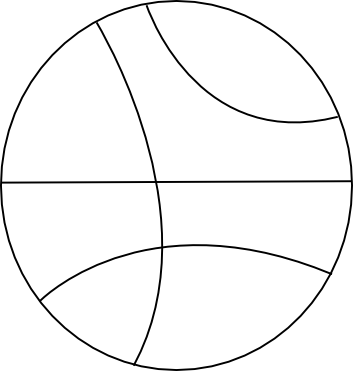
\includegraphics[width=0.5\textwidth]{PoincareDisc.png}
	\caption[A visualisation of the two dimensional Poincar\'{e} disc model containing four geodesics]{A visualisation of the two dimensional Poincar\'{e} disc model containing four geodesics \protect{\cite{poincare_model_web_page}}.}
	\label{fig:poincare_example}
\end{figure}

An example of this is shown in figure \ref{fig:poincare_example}. Here, four separate geodesics have been drawn on a hyperbolic plane and then visualised in Euclidean space using the disc model. Though these lines do not appear straight in Euclidean space the negative curvature of the hyperbolic space causes their apparent curvature in this model. Any geodesics which do not intersect inside the disc are considered parallel.

Measuring a Euclidean angle in this model yields the actual Hyperbolic angle thus making the model conformal. Angles are determined by simply measuring the angle between the tangents of the Euclidean representation of the curves at the point of intersection. This property of the model makes it extremely useful for visualisations where angles are important.

Calculating Hyperbolic distance in the disc model is more complex than simply measuring distances in the Euclidean representation. Hyperbolic distance in the disc model, between the Euclidean points A and B, is defined as \cite{blair_inversion_2000}:

\begin{equation}
\label{distance_disc_model}
\log(AB,PQ)
\end{equation}

where P and Q are the ideal points of the geodesic that bisects A and B. These points must be in the order P, B, A, Q on the line. (AB, PQ) is the \textit{cross-ratio} of the four points and is defined as \cite{blair_inversion_2000}:

\begin{equation}
\label{cross_ratio}
(AB,PQ) = \frac{|AP|\cdot|BQ|}{|BP|\cdot|AQ|}
\end{equation}

where |PQ|, for example, is the Euclidean arc length between the points P and Q on the Euclidean representation of the Hyperbolic line which intersects A and B.

The further an object is from the centre of the space the more compressed it's Euclidean representation becomes, making it appear smaller. Objects near the centre of the space are represented more accurately as the compression of the Hyperbolic space is low there.

\subsection{The Beltrami-Klein Model}

The Beltrami-Klein model of hyperbolic geometry, known henceforth as the \textit{projective model} addresses the issue of the distortion of the "straightness" of lines but introduces a distortion of angle.

The projective model is again defined in two-dimensional Euclidean space as the open unit disc, given earlier in equation \ref{eq:open_unit_disc_eq}. A geodesic, in the projective model is any chord of the unit disc. Indeed, for a geodesic in the disc model which has ideal points A and B it is trivial to determine the equivalent in the projective model, it is simply the chord AB.

The method for calculating distance in the projective model differs slightly from the disc model and the distance between points A and B is defined as \cite{milnor_hyperbolic_1982}:

\begin{equation}
\label{distance_disc_model}
\frac{1}{2}\log(AB,PQ)
\end{equation}

Where P and Q are again the ideal endpoints of the geodesic that intersects A and B and all four points are defined on the line in the order P, B, A, Q. (AB, PQ) is the cross-ratio of the four points as defined in equation \ref{cross_ratio}.

\begin{figure}
	\centering
	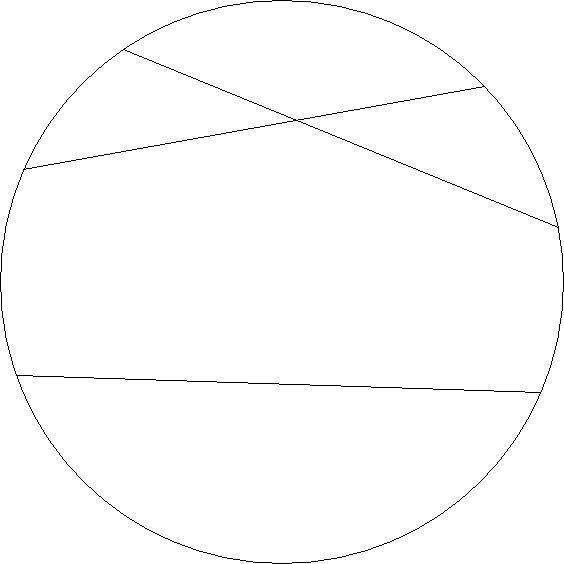
\includegraphics[width=0.5\textwidth]{Klein_model.png}
	\caption[A visualisation of the two dimensional Beltrami-Klein model containing three geodesics]{A visualisation of the two dimensional Beltrami-Klein model containing three geodesics \protect{\cite{klein_model_image}}.}
	\label{fig:klein_example}
\end{figure}

Figure \ref{fig:klein_example} provides an example of the model containing three geodesics. If two geodesics do not intersect within the  In this diagram the two topmost lines are parallel to the bottommost line and both pass through the same point, an important property of hyperbolic space. As the Hyperbolic space is effectively bent in the visualisation, Euclidean angles in this model do not correspond to the same Hyperbolic angles and this must be accounted for if the correct modelling of angles is important, as such the model is not conformal. Of course, if it is unimportant for angles to be accurate in the visualisation then this model may be ideal.

As the model is not conformal, it is difficult to measure Hyperbolic angles given only the Euclidean representation of the model. Instead of attempting to measure angles directly, it is far more simple to convert to a conformal model and measure Euclidean angles directly. Fortunately, a simple conversion exists from the projective model to the disc model:

\begin{equation}
\label{projective_to_disc}
u=\frac{(1-\sqrt{1-s\cdot{}s})s}{s\cdot{}s}
\end{equation}

Where $s$ is a vector representing a point in the projective model and $u$ is its equivalent in the disc model. A similar conversion exists in the opposite direction and is given by:

\begin{equation}
\label{disc_to_projective}
s=\frac{2u}{1+u\cdot{}u}
\end{equation}

As the models are related by these simple equations conversion between them is trivial. Of course, any geodesic can be easily converted between the models by using its ideal points, simplifying conversion between the two models further.

It is important to note that both the disc and projective models map Hyperbolic space to Euclidean space in such a way that changing the position of the centre of the visualisation will alter the Euclidean size of objects shown. This property effectively allows for a focus on a specific object, which will appear in the centre of the visualisation at its actual Hyperbolic size but also gives a view of the entire space with objects being scaled down in size more the further they are from the centre. This property of these visualisations is extremely useful for displaying trees which have high branch factors, a property that is exhibited by graph representations of the internet.

\subsection{The Poincar\'{e} Half-Plane Model}

Both models discussed previously represent the infinite hyperbolic plane inside a finite Euclidean circle, the Poincar\'{e} half-plane model, known henceforth as the \textit{half-plane} model, does not. Instead, the infinite hyperbolic space is plotted in the upper-half plane, defined as \cite{kubo_geometry_1988}:

\begin{equation}
\label{upper_half_plane}
\{(x,y):y>0\}
\end{equation}

Unlike the previous two models, the half-plane model is unbounded in the x direction, providing infinite space in which to visualise Hyperbolic space. However, a bounding still exists in the y direction, which, like previous models, compresses the space infinitely at the bound. Ideal points lie on the line $y=0$ which are again infinitely far from all other points.

As the space is infinite in the x and positive-y directions geodesics appear quite differently to the disc and projective models. A geodesic in the half-plane model appears as either a Euclidean circular arc perpendicular to the x-axis or as a straight line perpendicular to the x-axis. Lines are parallel if they do not intersect in the plane.
\begin{figure}
	\centering
	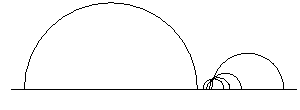
\includegraphics[width=0.75\textwidth]{upper-half-plane.png}
	\caption[A visualisation of the two dimensional Poincar\'{e} half-plane model containing five geodesics]{A visualisation of the two dimensional Poincar\'{e} half-plane model containing five geodesics \protect{\cite{half_plane_example}}.}
	\label{fig:half-plane-example}
\end{figure}

Figure \ref{fig:half-plane-example} shows an example of the half-plane model in which five geodesics have been plotted. In this example all of the lines on the right are parallel to the leftmost line, additionally the lines on the right also intersect at a single point.

Measuring the distance between points in the half-plane model is more complex than the previous two and is defined as \cite{kubo_geometry_1988}:

\begin{equation}
\label{half_plane_distance}
arcosh\left(1+\frac{(x_2-x_1)^2+(y_2-y_1)^2}{2y_1y_2}\right)
\end{equation}

Where the points are given in the form $(x_1, x_2), (y_1, y_2)$, unlike the previous models which use pure vector mathematics. Measuring angles is simple, however, as the model is conformal, simply measuring the Euclidean angle between the tangents of the lines at the point of intersection yields the Hyperbolic angle.

An interesting property of the half-plane model is the appearance of circles in the model, they appear as Euclidean circles. Though this may seem strange the appearance of the circle is deceiving as its Hyperbolic centre is not equivalent to its Euclidean centre. A Hyperbolic circle with centre $(x,y)$ and radius $R$ is modelled by a Euclidean circle with centre $(x, y \cosh R)$ and radius $y \sinh R$. This conformance of circles makes the half-plane model a good choice for representations which include Hyperbolic circles, but one must be wary of the distortion of the centre of such circles.

\section{Embedding Methods}
In order to be able to produce a visualisation of Hyperbolic space it is first necessary to determine how the chosen data lies in such a space. This process is known as \textit{embedding} and will be discussed in this section.

\subsection{A Greedy Embedding Method}

Cvetkovski et al. \cite{cvetkovski_hyperbolic_2009} describe a method for embedding dynamic graphs into Hyperbolic space for the purposes of routing. This implementation uses the Poincar\'{e} disc model. Focussing on trees, this method selects a root location in the space at which to place the root node of the tree subject to constraints which cause the node to be placed at an optimal location in the space. The method relies on the network nodes themselves electing a root node and subsequently forming a minimal-depth tree. The nodes accomplish this by each selecting a parent node to be the node that is the closest in hops to the root node. 

After the nodes have identified their parents, the root node is plotted into the space at the chosen location and each node calculates its position in the embedding relative to its parent node. This calculation is performed by initialising two angles for the root node $\alpha_r = \pi$ and $\beta_r = 2\pi$ which correspond to ideal points. A node, $n$, to be placed in the embedding receives angles $\alpha_n = \alpha_p$ and $\beta_n = (\alpha_p + \beta_p) /2$ from its parent, $p$, and determines its own position in the embedding by reflecting the position of it's parent (in this case the root node) in the geodesic $G$ constructed between $\alpha_n$ and $\beta_n$ After sending $\alpha_n$ and $\beta_rn$ to the child the parent node updates the value $\alpha_p := \beta_n$. This method of updating these values ensures there is unlimited space available for the expansion of the tree. This process in then repeated for each node to form a greedy embedding. 

This method of creating an embedding, while offering guaranteed success due to its greedy implementation, has some flaws. The real, physical locations of the nodes are not represented in the embedding, something which is important to the aims of this project. Further, the embedding is designed to be used for a greedy routing algorithm described in the same work, which limits its usefulness when applied to the problem for this project. Indeed, the embedding produces a tree which is not indicative of all links between all nodes and would therefore misrepresent the data. Despite these flaws, the approach of performing an embedding in this way is an interesting application of knowledge and does give some useful insight into the practical uses for such embeddings. 

\subsection{H3: Large Directed Graphs in Hyperbolic Space}

Munzner \cite{munzner_h3_1997} describes a method for laying out large directed graphs in Hyperbolic space. This implementation uses a three dimensional version of the Beltrami-Klein model. The method once again operates on trees but it is possible to display further links between nodes once the model has been plotted. Though a root node must be chosen and a spanning tree constructed, it is possible to use this method to visualise an undirected graph accurately. 

The basis of the method uses \textit{spherical caps} to lay out the nodes in the Hyperbolic space. Each node has a cap with size proportional to the number of nodes descended from it in the tree. This includes all descendant nodes, not just immediate child nodes. These caps represent the area required to embed all descendant nodes of the node to which the cap belongs. As Hyperbolic space expands in all directions, it is possible to fit more caps of equivalent size into the space further down the tree. This allows trees with high branch factor to be embedded into the space easily.

The algorithm to place the caps functions recursively; it first computes the size of the caps required for all leaf nodes, which have a fixed cap size due to having no children, which is the base case for the algorithm. The algorithm then traverses back up the tree and computes the area required for the cap belonging to each node, taking into account the cap size of all child nodes. Finally, the cap size for the root node is calculated, which is the total size of the embedding. Though the size of the caps has been calculated at this point, they have not been laid out in the space, this is the next function of the algorithm, which iterates down the tree from the root node laying out each child cap of each node, until all caps have been placed. This is accomplished through \textit{sphere-packing}, a common mathematical problem outlined by Hales in 1992 \cite{hales_sphere_1992}.

While this method seems more appropriate than the previous one, it does present issues when combined with the aims of this project. Once again, the embedding does not take into account the physical locations of the nodes, indeed the examples supplied in the paper are those without such locations like files in a file system. Though the method could be adapted to take physical location into account, it would be far more appropriate to use a method designed to do this from the beginning. Though it may appear that it is possible to embed a graph using this model the embedding would distort the distances between the nodes even if it was converted to account for physical location. Due to the original embedding being constructed using the tree any links which did not appear in this tree would be vastly distorted, making the embedding misleading. Though the technique of using spherical caps and sphere packing to perform the embedding is efficient, the limitations of this method as a whole decrease its viability for use in this project.

\subsection{A More Mathematical Hyperbolic Embedding Method}

So far, the methods discussed to perform an embedding have been of the practical, algorithmic variety. The method outlined by Wilson et al. \cite{wilson_spherical_2014} is a more mathematical method. This method uses the matrix describing the distances between points in Euclidean space, which should correspond to the distances in Hyperbolic space, to produce a embedding of points in Hyperbolic space.

This method uses the inner product of the points, defined for Hyperbolic space as: 

\begin{equation}
\label{eq:inner_product_hyperbolic}
\langle x_i,x_j\rangle = -r^2\cosh \left(\frac{d_{ij}}{r}\right)
\end{equation}

where $r$ is the radius of the embedding space and $d_{ij}$ is the distance between a pair of points $i$ and $j$. It is possible to calculate $\boldsymbol{Z}$, the inner product of the points, directly from this equation, but this is not possible immediately as the radius, $r$, is unknown. As $\boldsymbol{Z}$ is an inner product matrix of points in Hyperbolic space it should have exactly one negative eigenvalue and one zero eigenvalue. This is due to hyperbolic space having a single negative dimension. Knowing this, it is possible to minimise the magnitude of the second smallest eigenvalue to find $r$ by:

\begin{equation}
\label{eq:argmin_hyperbolic}
r^*=\underset{r}{\arg\min}|\lambda_2[\boldsymbol{Z}(r)]|
\end{equation}

where $\lambda_2$ is the value of the second smallest eigenvalue of $\boldsymbol{Z}$. Having approximated $r$ it is then possible to calculate $\boldsymbol{Z}$ using equation \ref{eq:inner_product_hyperbolic}, this then allows for the calculation of $\boldsymbol{X}$, the point matrix for a Euclidean embedding of the space, through eigendecomposition of $\boldsymbol{Z}$ to obtain a matrix of its eigenvalues, $\boldsymbol{\Lambda}$ and a matrix of its eigenvectors $\boldsymbol{U}$. It is then possible to calculate $\boldsymbol{X}$ by:

\begin{equation}
\label{eq:embedding_x}
\boldsymbol{X}=\boldsymbol{U}_Z\boldsymbol{\Lambda}_{z||}^{\frac{1}{2}}
\end{equation}

The result of this equation is an $NxN$ matrix for which each row is a point and each column represents a dimension of the embedding. As with a standard embedding, it is possible to drop any dimensions which have negative eigenvalues, yielding a co-ordinate matrix that specifies the Hyperbolic co-ordinates of the points.

This method is vastly superior to those previously discussed, its primary advantage arises from the strategy of embedding using pre-existing geometric data. In the case of this project, this allows the embedding to use location data gathered for ASes without having to adapt the embedding method. Further, this method is already generalised to any number of dimensions, meaning it is possible to produce both two and three dimensional representations of the data. 

\section{Haversine Formula}
When considering the locations of ASes on the Earth's surface a suitable system must be used, the most obvious and simple of which is the latitude longitude geographic co-ordinate system (henceforth known as lat-long). As this system can effectively map any point on the Earth's surface and is well known and understood it is an easy choice to make. However, a key requirement of the chosen system is that it is possible to easily determine distances, something which lat-long fails to provide. It is insufficient to simply treat the lat-long co-ordinates as absolute positions and calculate distance through the difference between the co-ordinates as the earth is not flat. Instead a method known as the Haversine formula must be used.

The Haversine formula calculates the distance between two points on the surface of a sphere and is defined as \cite{chopde_landmark_2013}:

\begin{equation}
\label{haversine_formula}
2r\sin^-1\left(\sqrt{\sin^2\left(\frac{\phi_2 - \phi_1}{2}\right) + \cos(\phi_1) \cos(\phi_2) \sin^2\left(\frac{\psi_2 - \psi_1}{2}\right)}\right)
\end{equation}

where a pair of points are given with latitude and longitude $(\phi,\psi)$ and $r$ is the radius of the Earth. 

Though the computed distance may not be exact due to the Earth not being a uniform sphere, it is satisfactory for the purposes of this project.